\documentclass[12pt,a4paper]{article}
\usepackage{ucebnice}

\usetikzlibrary{hobby}

% FUNKCE PRO KRESLENÍ ČAR

\newcommand{\japanesemultiplication}[3][]{%

    \def\splitfirst##1##2\relax{
        \def\firsttens{##1}
        \def\firstones{##2}
    }
    \def\splitsecnd##1##2\relax{
        \def\secndtens{##1}
        \def\secndones{##2}
    }
    \splitfirst#2\relax
    \splitsecnd#3\relax
    
    \tikzset{
        canvas/.style={rotate=135},
        first number/.style={blue},
        second number/.style={red},
        crossing/.style={fill, circle},
        group/.style={thick, black},
        first group/.style={},
        second group/.style={},
        third group/.style={},
        digit/.style={font=\Huge},
        first digit/.style={left of=one},
        second digit/.style={below of=min},
        third digit/.style={right of=two},
    }

    \begin{tikzpicture}[#1]
        \begin{scope}[canvas]
            \foreach \x in {1,...,\firsttens} {
                \draw[first number] ({1+\x},-10) -- ({1+\x},10);
            }
            \foreach \x in {1,...,\firstones} {
                \draw[first number] ({-1-\x},-10) -- ({-1-\x},10);
            }
            \foreach \y in {1,...,\secndtens} {
                \draw[second number] (-10,{1+\y}) -- (10,{1+\y});
            }
            \foreach \y in {1,...,\secndones} {
                \draw[second number] (-10,{-1-\y}) -- (10,{-1-\y});
            }
            \foreach \x in {1,...,\firsttens} {
                \foreach \y in {1,...,\secndtens} {
                    \node[crossing] (a\x\y) at ({1+\x},{1+\y}) {};
                }
                \foreach \y in {1,...,\secndones} {
                    \node[crossing] (b\x\y) at ({1+\x},{-1-\y}) {};
                }
            }
            \foreach \x in {1,...,\firstones} {
                \foreach \y in {1,...,\secndtens} {
                    \node[crossing] (c\x\y) at ({-1-\x},{1+\y}) {};
                }
                \foreach \y in {1,...,\secndones} {
                    \node[crossing] (d\x\y) at ({-1-\x},{-1-\y}) {};
                }
            }
            \coordinate (max) at ({1.5+\firsttens},{-1.5-\secndones});
            \coordinate (maxr) at ({1+\firsttens},-1);
            \coordinate (maxl) at (1,{-1-\secndones});
            \coordinate (min) at ({-1.5-\firstones},{1.5+\secndtens});   
            \coordinate (minr) at (-1,{1+\secndtens});   
            \coordinate (minl) at ({-1-\firstones},1);
            \coordinate (null) at (-.5,-.5);
            \coordinate (nulr) at (.5,.5);
            
            \coordinate (one) at ({1+\firsttens},{1+\secndtens});
            \coordinate (onea) at (1,11);
            \coordinate (oneb) at (1,6);
            \coordinate (onec) at (1,1);
            \coordinate (oned) at (6,1);
            \coordinate (onee) at (11,1);
    
            \coordinate (two) at ({-1-\firstones},{-1-\secndones});
            \coordinate (twoa) at (-1,-11);
            \coordinate (twob) at (-1,-6);
            \coordinate (twoc) at (-1,-1);
            \coordinate (twod) at (-6,-1);
            \coordinate (twoe) at (-11,-1);
        \end{scope}
    
        \draw[group, second group] (max) to[closed, curve through={(maxl) .. (null) .. (minl) .. (min) .. (minr) .. (nulr) .. (maxr)}] cycle;
    
        \draw[group, first group] (onea) to[curve through={(oneb) .. (onec) .. (oned)}] (onee);
    
        \draw[group, third group] (twoa) to[curve through={(twob) .. (twoc) .. (twod)}] (twoe);
        
        \node[digit, first digit] {%
            \pgfmathparse{\firsttens*\secndtens}%
            \pgfmathprintnumber{\pgfmathresult}%
        };
        
        \node[digit, second digit] {%
            \pgfmathparse{\firsttens*\secndones+\secndtens*\firstones}%
            \pgfmathprintnumber{\pgfmathresult}%
        };

        \node[digit, third digit] {%
            \pgfmathparse{\firstones*\secndones}%
            \pgfmathprintnumber{\pgfmathresult}%
        };

    \end{tikzpicture}
}



\title{Základní matematické poznatky}
\author{Ondřej Škubala}
\date{\today}

\begin{document}

\maketitle
\newpage

\section{Elementární teorie čísel}

% Úvod kapitoly
% Úvod kapitoly
\begin{quotebox}
{„Matematika je královnou věd a teorie čísel královnou matematiky.“}
{Carl Friedrich Gauss}
\end{quotebox}

\noindent
V této kapitole se poprvé setkáme s \emph{elementární teorií čísel}.  
Budeme zkoumat základní vlastnosti přirozených a celých čísel – jak se zapisují, jak se dělí, co znamená, že jedno číslo je násobkem druhého, a co jsou to prvočísla nebo složená čísla.  
Ukážeme si také, jak lze čísla rozkládat na součin prvočísel, jak hledat jejich společné dělitele a násobky a proč jsou tyto pojmy důležité nejen v matematice, ale i v běžném životě.  


\begin{historicalbox}
Studium vlastností čísel patří mezi nejstarší matematické disciplíny. Již starověké civilizace se zabývaly otázkami dělitelnosti, prvočísel a rozkladu čísel na součin menších částí.

\smallskip
\textbf{Starověký Egypt a Mezopotámie.}  
Egypťané využívali číselné znalosti při stavbě pyramid i při správě zásob obilí. Uměli rozkládat zlomky na součet jednotkových zlomků (např. $\tfrac{2}{3} = \tfrac{1}{2} + \tfrac{1}{6}$), což vyžadovalo cit pro dělitelnost čísel. Babyloňané zase používali poziční číselnou soustavu se základem $60$, díky které se dochovaly např. tabulky násobků a odmocnin.

\smallskip
\textbf{Řecko.}  
Největší rozkvět nastal u řeckých matematiků. \textbf{Pythagorejci} (6. stol. př. n. l.) považovali čísla za samotnou podstatu světa a přisuzovali jim mystický význam. Rozlišovali čísla sudá a lichá, dokonalá (např. $6 = 1+2+3$) a nedokonalá.  

\smallskip
\textbf{Eukleidés} (asi 300 př. n. l.) v díle \emph{Základy} shrnul systematicky veškeré tehdejší poznatky. Dokázal například, že existuje nekonečně mnoho prvočísel, a popsal algoritmus pro hledání největšího společného dělitele — dnes známý jako \emph{Eukleidův algoritmus}.  

\smallskip
\textbf{Eratosthenés} (kolem 200 př. n. l.) představil tzv. \emph{síto Eratosthenovo}, jednoduchý postup k nalezení prvočísel menších než zvolené číslo.  

\smallskip
\textbf{Diofantos} (3. stol. n. l.) je považován za „otce algebraické teorie čísel“. Ve svém díle \emph{Aritmetika} řešil rovnice, kde se hledají celočíselná řešení (tzv. diofantické rovnice).

\smallskip

\smallskip

\smallskip

\smallskip

\smallskip

\smallskip

\smallskip
\textbf{Středověk a arabský svět.}  
Po pádu Říma převzali štafetu učenci v arabském světě. \textbf{Al-Chvárizmí} (9. stol.) sepsal práce o aritmetice a algebraických postupech, které se dostaly do Evropy a položily základy moderní algebry. Arabové rozšířili používání indicko-arabských číslic a poziční desítkové soustavy.

\smallskip
\textbf{Evropa novověku.}  
Od 17. století se teorie čísel stala vážným vědeckým oborem. \textbf{Pierre de Fermat} (1607–1665) formuloval řadu tvrzení, z nichž slavná \emph{malá Fermatova věta} se stala klíčovým nástrojem v moderní teorii čísel. Jeho \emph{poslední věta} (že rovnice $x^n+y^n=z^n$ nemá pro $n>2$ nenulová celočíselná řešení) byla dokázána až v roce 1994 Andrewem Wilesem.  

\smallskip
\textbf{Leonhard Euler} (1707–1783) významně rozvinul teorii kongruencí a zavedl např. \emph{Eulerovu funkci} $\varphi(n)$, která počítá počet čísel nesoudělných s $n$.  

\smallskip
\textbf{Carl Friedrich Gauss} (1777–1855) vydal slavné dílo \emph{Disquisitiones Arithmeticae} (1801), které položilo základy moderní teorie čísel a systematicky rozvinulo teorii kongruencí.

\smallskip
\textbf{19. a 20. století.}  
V 19. století se začala teorie čísel dělit na elementární a algebraickou. Objevily se nové oblasti: studium prvočíselné funkce, Lagrangeovy a Legendreovy výsledky o kvadratických zbytcích, Riemannova hypotéza (1859) a další.  

Ve 20. století a dál se teorie čísel stala i praktickým nástrojem — například pro kryptografii (RSA, Diffie-Hellman), kompresi dat či teorii kódování. Využívá se v informatice, při zabezpečení internetu a při šifrování dat.

\smallskip
\textbf{Shrnutí.}  
Elementární teorie čísel tedy spojuje více než 3000 let starou tradici lidského poznání s moderními aplikacemi, které dnes každý den používáme, aniž si to uvědomujeme.
\end{historicalbox}


\subsection{Zápis přirozených čísel}

Přirozená čísla zapisujeme v \emph{desítkové (dekadické) soustavě}, která používá základ $10$ a cifry $0$ až $9$.  
Každé přirozené číslo lze zapsat jako součet mocnin desítky vynásobených příslušnými ciframi. Tento způsob se nazývá \emph{rozvinutý zápis čísla}.  

\[
150 = 1 \cdot 10^2 + 5 \cdot 10^1 + 0 \cdot 10^0
\]

\[
2025 = 2 \cdot 10^3 + 0 \cdot 10^2 + 2 \cdot 10^1 + 5 \cdot 10^0
\]

Rozvinutý zápis nám ukazuje, jak číslo vzniká skládáním násobků mocnin desítky.  



\subsection{Znaky dělitelnosti}
\subsubsection*{Násobky a dělitelnost čísel}
Řekneme, že číslo $a$ je \emph{násobkem} čísla $b$ (a tedy číslo $b$ je \emph{dělitelem} čísla $a$), právě tehdy, když existuje celé číslo $k$, pro které platí:
\[
a = k \cdot b.
\]

Tento vztah zapisujeme také zkráceně:
\[
b \mid a,
\]
což čteme „$b$ dělí $a$“.  
Pokud číslo $b$ nedělí číslo $a$, zapisujeme to symbolem
\[
b \nmid a.
\]


\subsubsection*{Znaky dělitelnosti}

Při práci s čísly často potřebujeme rychle zjistit, zda je nějaké číslo dělitelné určitým jiným číslem.  
U menších čísel to dokážeme z hlavy nebo si můžeme udělat krátký rozklad.  
Ale u větších čísel by bylo zdlouhavé pořád počítat. Proto se v matematice objevila jednoduchá pravidla, kterým říkáme \emph{znaky dělitelnosti}.  

Každý znak je vlastně „trik“, který nám umožní určit dělitelnost jen pohledem na cifry nebo jednoduchým výpočtem.  
Například místo toho, abychom složitě dělili číslo $372$ třemi, sečteme jeho cifry ($3+7+2=12$) a poznáme, že je dělitelné $3$.  
Takových pravidel existuje více a některá jsou opravdu elegantní.  
Níže jsou sepsána nejznámější pravidla pro dělitelnost čísly $2$ až $11$. 

\subsubsection*{Dělitelnost dvěma}
Číslo je dělitelné $2$, jestliže jeho poslední cifra je sudá (tj. $0,2,4,6,8$).  

\begin{examplebox}
Číslo $246$ je dělitelné $2$, protože končí cifrou $6$.  
Číslo $375$ není dělitelné $2$, protože končí cifrou $5$.
\end{examplebox}

\subsubsection*{Dělitelnost třemi}
Číslo je dělitelné $3$, jestliže součet jeho cifer je dělitelný $3$.  

\begin{examplebox}
Číslo $372$ je dělitelné $3$, protože $3+7+2=12$ a $12$ je dělitelné $3$.  
Číslo $745$ není dělitelné $3$, protože $7+4+5=16$ a $16$ dělitelné $3$ není.
\end{examplebox}

\subsubsection*{Dělitelnost čtyřmi}
Číslo je dělitelné $4$, jestliže jeho poslední dvě cifry tvoří číslo dělitelné $4$.  

\begin{examplebox}
Číslo $516$ je dělitelné $4$, protože poslední dvě cifry tvoří $16$, které je dělitelné $4$.  
Číslo $527$ není dělitelné $4$, protože $27$ dělitelné $4$ není.
\end{examplebox}

\subsubsection*{Dělitelnost pěti}
Číslo je dělitelné $5$, jestliže končí cifrou $0$ nebo $5$.  

\begin{examplebox}
Číslo $2\,735$ je dělitelné $5$, protože končí cifrou $5$.  
Číslo $2\,738$ není dělitelné $5$, protože končí cifrou $8$.
\end{examplebox}

\subsubsection*{Dělitelnost šesti}
Číslo je dělitelné $6$, jestliže je současně dělitelné $2$ a $3$.  

\begin{examplebox}
Číslo $84$ je dělitelné $6$, protože je sudé a zároveň $8+4=12$, což je dělitelné $3$.  
Číslo $82$ není dělitelné $6$, protože sice je sudé, ale $8+2=10$, což dělitelné $3$ není.
\end{examplebox}


\subsubsection*{Dělitelnost sedmi}
Číslo je dělitelné $7$, jestliže po odečtení dvojnásobku poslední cifry od zbytku čísla dostaneme číslo dělitelné $7$.  
(Tento znak se používá méně často, protože je složitější.)  

\begin{examplebox}
Číslo $203$ je dělitelné $7$, protože $20 - 2 \cdot 3 = 14$, a $14$ je dělitelné $7$.  
Číslo $205$ není dělitelné $7$, protože $20 - 2 \cdot 5 = 10$, a $10$ dělitelné $7$ není.
\end{examplebox}

\subsubsection*{Dělitelnost osmi}
Číslo je dělitelné $8$, jestliže jeho poslední tři cifry tvoří číslo dělitelné $8$.  

\begin{examplebox}
Číslo $7\,432$ je dělitelné $8$, protože poslední tři cifry tvoří $432$, a $432 \div 8 = 54$.  
Číslo $7\,434$ není dělitelné $8$, protože $434 \div 8 = 54{,}25$.
\end{examplebox}

\subsubsection*{Dělitelnost devíti}
Číslo je dělitelné $9$, jestliže součet jeho cifer je dělitelný $9$.  

\begin{examplebox}
Číslo $2\,511$ je dělitelné $9$, protože $2+5+1+1=9$, a $9$ je dělitelné $9$.  
Číslo $2\,512$ není dělitelné $9$, protože $2+5+1+2=10$.
\end{examplebox}

\subsubsection*{Dělitelnost deseti}
Číslo je dělitelné $10$, jestliže končí cifrou $0$.  

\begin{examplebox}
Číslo $3\,470$ je dělitelné $10$, protože končí nulou.  
Číslo $3\,471$ není dělitelné $10$, protože končí cifrou $1$.
\end{examplebox}

\subsubsection*{Dělitelnost jedenácti}
Číslo je dělitelné $11$, jestliže rozdíl součtu cifer na lichých a sudých pozicích je dělitelný $11$.  

\begin{examplebox}
Číslo $6\,281$ je dělitelné $11$, protože $(6+8) - (2+1) = 11$, a $11$ je dělitelné $11$.  
Číslo $6\,282$ není dělitelné $11$, protože $(6+8) - (2+2) = 10$, což $11$ nedělí.
\end{examplebox}

\subsection{Soudělná a nesoudělná čísla}

Znakům dělitelnosti rozumíme už celkem dobře. Nyní se můžeme posunout o krok dál:  
budeme se ptát, jak to vypadá, když porovnáváme více čísel mezi sebou.  

Dvě nebo více přirozených čísel mohou mít společné dělitele.  
Pokud mají kromě čísla $1$ ještě nějakého dalšího společného dělitele, nazýváme je \emph{soudělná čísla}.  
Naopak, jestliže jejich jediným společným dělitelem je $1$, nazýváme je \emph{nesoudělná čísla}.  

Jinými slovy:  
\begin{itemize}
    \item Soudělná čísla mají „více společného“ – například $18$ a $24$ jsou soudělná, protože je dělí $2$, $3$ i $6$.  
    \item Nesoudělná čísla jsou naopak „nezávislá“ – například $8$ a $15$ mají jediného společného dělitele, a to $1$.  
\end{itemize}

\begin{examplebox}
\begin{itemize}
    \item $18$ a $24$ jsou \textbf{soudělná}, protože mají společné dělitele $1,2,3,6$.  
    \item $8$ a $15$ jsou \textbf{nesoudělná}, protože jejich jediným společným dělitelem je $1$.  
    \item $21$ a $35$ jsou \textbf{soudělná}, protože mají společné dělitele $1$ a $7$.  
\end{itemize}
\end{examplebox}

\begin{notebox}
Soudělnost a nesoudělnost hrají důležitou roli při práci s dělitelností.  
Například při hledání \emph{největšího společného dělitele (NSD)} nebo \emph{nejmenšího společného násobku (NSN)}.  
Pokud jsou čísla nesoudělná, je jejich NSD vždy $1$.  
Naopak u soudělných čísel je NSD větší než $1$ a určuje, jak velké „kousky“ mají čísla společné.  
\end{notebox}

\noindent
Znalost soudělnosti a nesoudělnosti čísel hraje důležitou roli například při hledání \emph{největšího společného dělitele} (NSD) nebo při určování, zda lze dvě veličiny rozdělit beze zbytku na stejné části.

\newpage
\section{Triky pro násobení čísel}

\begin{quotebox}
{„Žádná část matematiky není ušlechtilejší než teorie čísel.“}
{G. H. Hardy}
\end{quotebox}

V dějinách matematiky se objevila řada zajímavých postupů, jak si usnadnit násobení.  
Některé se předávají jako lidové „kouzelnické triky“, jiné byly kdysi vážně používanými metodami výpočtu.  
Uvedeme si několik ukázek.

\subsubsection*{Trik s číslem 9 (na prstech)}
Chcete-li vynásobit $9$ čísly $1$ až $10$, stačí položit obě ruce dlaněmi dolů a ohýbat příslušný prst.  
\begin{examplebox}
\begin{itemize}
    \item Pro $9\cdot 3$ ohneme třetí prst; vlevo od něj zůstávají $2$ prsty (desítky), vpravo $7$ prstů (jednotky). Výsledek: $27$.
    \item Pro $9\cdot 6$ ohneme šestý prst; vlevo $5$, vpravo $4$. Výsledek: $54$.
\end{itemize}
\end{examplebox}

\subsubsection*{Násobení blízkých čísel}
Pokud se obě čísla liší jen málo od nějaké základny (např. $100$), lze násobit snadno pomocí rozkladu.  
\begin{examplebox}
\[
98\cdot 97 = (100-2)(100-3) = 100^2 - 100\cdot(2+3) + 6 = \mathbf{9\,506}.
\]
\end{examplebox}

\subsubsection*{Metoda kosodélníku (lattice method)}

Tento postup se využíval už ve středověku a objevuje se i v moderní výuce matematiky (např. v \emph{Hejného metodě}).  
Čísla se zapíší do mřížky (kosodélníkové „pole“), v každém políčku se zapíše dílčí součin a pak se sčítají úhlopříčky.  

\begin{center}
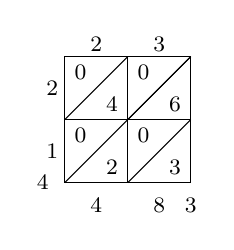
\begin{tikzpicture}[scale=0.8, every node/.style={font=\footnotesize}]
  % čtverce s diagonálami
  \draw (0,0) rectangle (1,1);
  \draw (1,0) rectangle (2,1);
  \draw (0,1) rectangle (1,2);
  \draw (1,1) rectangle (2,2);

  % diagonály
  \draw (0,1) -- (1,2);
  \draw (1,1) -- (2,2);
  \draw (0,0) -- (2,2);
  \draw (1,0) -- (2,1);

  % popisky čísel (23 × 21)
  \node at (0.5,2.2) {2};
  \node at (1.5,2.2) {3};
  \node at (-0.2,1.5) {2};
  \node at (-0.2,0.5) {1};

  % součiny v buňkách
  \node at (0.25,1.75) {0};
  \node at (0.75,1.25) {4};
  \node at (1.25,1.75) {0};
  \node at (1.75,1.25) {6};
  \node at (0.25,0.75) {0};
  \node at (0.75,0.25) {2};
  \node at (1.25,0.75) {0};
  \node at (1.75,0.25) {3};

  % výsledky po diagonálách
  \node[below] at (2,-0.1) {3};
  \node[below] at (1.5,-0.1) {8};
  \node[below] at (0.5,-0.1) {4};
  \node[left]  at (-0.1,0) {4};
\end{tikzpicture}
\end{center}

Sečtením diagonál dostáváme výsledek:
\[
23 \cdot 21 = 483.
\]

\begin{notebox}
\begin{itemize}
    \item \textbf{Výhoda:} minimalizuje zátěž krátkodobé paměti při výpočtu – je třeba méně mentálních úkonů.  
    \item Grafická úprava zápisu je vhodná i pro hledání společných dělitelů či násobků čísel.  
    \item \textbf{Nevýhoda:} obtížnější orientace pro žáky s dysgrafií, protože algoritmus vyžaduje „náročnější“ kreslení struktury čísel – což ale může platit i pro jiné způsoby ručního násobení.  
    \item Tato metoda se objevuje také v \emph{Hejného metodě} jako prostředek k porozumění násobení.  
\end{itemize}
\end{notebox}


\subsubsection*{Japonské násobení čarami}
Existuje i netradiční způsob násobení, který se někdy označuje jako \emph{japonské násobení} nebo \emph{metoda čar}.  
Každá cifra se znázorní jako určitý počet rovnoběžných čar. Čáry jednoho činitele se kreslí šikmo zleva doprava, druhého šikmo zprava doleva.  
Výsledek vznikne sčítáním průsečíků v diagonálních pásmech.  

\begin{center}
\resizebox{7cm}{!}{\japanesemultiplication{42}{21}}
\end{center}
\begin{examplebox}
Průsečíky dávají jednotky, desítky a stovky. Výsledek:
\[
42 \cdot 21 = 8\cdot10^3 + 8\cdot10^2 + 2\cdot10^1 = 882.
\]
\end{examplebox}

\begin{center}
\resizebox{7cm}{!}{\japanesemultiplication{38}{26}}
\end{center}
\begin{examplebox}
Druhý příklad ukazuje $38 \cdot 26$, což dává
\[
38 \cdot 26 = 3\cdot10^3 + 6\cdot10^3 + 4\cdot10^2 + 4\cdot10^2 + 8\cdot10^1 = 988.
\]
\end{examplebox}

\subsubsection*{Indická metoda (védské násobení „křížem–svisle“) }

Tento postup vychází z tzv. \emph{védské matematiky}. A je dost podobná Japonské metodě násobemí čarami.
Výpočet se provádí ve třech krocích:
\begin{enumerate}[label=\arabic*.]
    \item \textbf{Jednotky:} vynásobíme poslední cifry.  
    \item \textbf{Křížem:} sečteme součiny „křížem“.  
    \item \textbf{Desítky:} vynásobíme první cifry.
\end{enumerate}

\begin{examplebox}
Počítejme $23 \cdot 12$.  
\begin{align*}
\text{Jednotky: } & 3 \cdot 2 = 6, \\
\text{Křížem: } & (2 \cdot 2) + (3 \cdot 1) = 7, \\
\text{Desítky: } & 2 \cdot 1 = 2.
\end{align*}
Sečtením dostáváme $276$.  
\end{examplebox}

Metodu lze snadno rozšířit i na víc než dvouciferná čísla.

\subsubsection*{Ruské násobení (tzv. egyptská metoda)}
Tento trik je známý i jako \emph{ruské násobení na půlky a dvojnásobky}.  
\begin{enumerate}[label=\arabic*.]
    \item Jedno číslo stále dělíme na polovinu (bez zbytku), druhé číslo stále zdvojnásobujeme.
    \item Pokračujeme, dokud první číslo neklesne na $1$.
    \item Výsledek je součet těch zdvojnásobených čísel, kde v prvním sloupci vyšlo liché číslo.
\end{enumerate}

\begin{examplebox}
Příklad: $23\cdot 12$
\[
\begin{array}{r|r}
23 & 12 \\
11 & 24 \\
5 & 48 \\
2 & 96 \\
1 & 192 \\
\end{array}
\]
Součet vybraných čísel je $12+24+48+192 = \mathbf{276}$.  
Opravdu $23\cdot 12 = 276$.
\end{examplebox}


\subsubsection*{Napoleonská metoda (násobení přes střed)}

Tento trik je velmi užitečný, pokud násobíme dvě čísla, která jsou „okolo“ nějakého zaokrouhleného čísla (např. $50$, $100$, $1000$).  
Obě čísla si představíme jako \emph{střed} $\pm$ \emph{odchylka}.  

\begin{examplebox}
Počítejme $47 \cdot 53$.  

Obě čísla jsou vzdálena o $3$ od středu $50$.  
Platí:
\[
47 \cdot 53 = 50^2 - 3^2 = 2500 - 9 = 2491.
\]

Rychlejší než běžný písemný postup!
\end{examplebox}


\subsubsection*{Geometrická metoda (obdélníkový model)}

Násobení lze také chápat jako výpočet \emph{obsahu obdélníku}.  
Každé číslo si rozdělíme na desítky a jednotky, vytvoříme menší obdélníky a jejich obsahy sečteme.  

\begin{examplebox}
Počítejme $23 \cdot 14$.  
Rozdělíme:
\[
23 = 20 + 3, \quad 14 = 10 + 4.
\]

Dílčí součiny:
\[
20 \cdot 10 = 200, \quad 20 \cdot 4 = 80, \quad 3 \cdot 10 = 30, \quad 3 \cdot 4 = 12.
\]

Sečteme:
\[
200 + 80 + 30 + 12 = 322.
\]

Násobení se tak promění na jednoduchý součet čtyř menších obdélníků.
\end{examplebox}

Tento přístup je součástí \emph{Hejného metody} a pomáhá žákům lépe chápat distributivní zákon a vztah mezi čísly.



\newpage
\section{Prvočísla a složená čísla}

% Na závěr kapitoly

\begin{quotebox}
{„Prvočísel je nekonečně mnoho.“}
{Eukleidés, Základy, Kniha IX, věta 20}
\end{quotebox}

\begin{historicalbox}
Prvočísla jsou jedním z nejstarších a nejtajemnějších objektů v celé matematice.  

\textbf{Starověk.}  
Už ve starověkém Řecku se prvočíslům věnovali Pythagorejci. \textbf{Eukleidés} (asi 300 př. n. l.) ve svém díle \emph{Základy} dokázal slavnou větu, že prvočísel je nekonečně mnoho – jednoduchým, ale geniálním důkazem.  
\textbf{Eratosthenés} (kolem 200 př. n. l.) zavedl \emph{síto Eratosthenovo}, postup, kterým lze systematicky „vyškrtávat“ složená čísla a tím získat seznam všech prvočísel do zvoleného limitu.  

\textbf{Středověk a arabský svět.}  
Arabští učenci přispěli k lepšímu chápání dělitelských vlastností čísel a zajímali se také o prvočísla. Do Evropy přinesli indicko-arabské číslice, díky nimž se výpočty s velkými čísly výrazně zjednodušily.  

\textbf{Novověk.}  
Od 17. století se studium prvočísel dostává na vyšší úroveň. \textbf{Pierre de Fermat} zkoumal tzv. Fermatova čísla a formuloval svou \emph{malou větu}.  
\textbf{Leonhard Euler} (18. století) objevil mnoho nových vlastností prvočísel, definoval Eulerovu funkci $\varphi(n)$ a dokázal, že existuje nekonečně mnoho prvočísel tvaru $4k+3$.  

\textbf{19. století.}  
\textbf{Carl Friedrich Gauss} se ve svém díle \emph{Disquisitiones Arithmeticae} (1801) věnoval mj. i prvočíslům a vyslovil (a později byla dokázána) tzv. \emph{věta o prvočíslech}, která říká, že prvočísla jsou s rostoucími čísly „řidší“, ale stále nekonečně mnohá.  
K tomuto období patří i \textbf{Adrien-Marie Legendre} a \textbf{Bernhard Riemann}, který v roce 1859 formuloval slavnou \emph{Riemannovu hypotézu} o rozložení prvočísel. Ta zůstává dosud nevyřešena a je jedním z největších problémů matematiky.  

\textbf{Současnost.}  
Dnes prvočísla nejsou jen předmětem čisté matematiky, ale mají obrovské praktické využití. Jsou klíčem k moderní kryptografii – například šifrovací systém \emph{RSA} je založen na tom, že rozložit velmi velké číslo na součin dvou prvočísel je pro počítače nesmírně obtížné.  
Největší známá prvočísla se hledají pomocí distribuovaných výpočtů a mají miliony číslic. Rekordy v hledání prvočísel se stále posouvají a ukazují, že i po tisících let bádání zůstávají prvočísla pro člověka tajemstvím i výzvou.  
\end{historicalbox}

\begin{definitionbox}
\textbf{Prvočíslo} je přirozené číslo větší než $1$, které má právě dva různé dělitele: číslo $1$ a sebe samo.
\end{definitionbox}

\begin{examplebox}
Prvočísla: $2, 3, 5, 7, 11, 13, 17, 19, 23, \dots$  

Není prvočíslo: $1$ (má pouze jednoho dělitele), $9$ (má dělitele $1, 3, 9$).
\end{examplebox}

\begin{definitionbox}
\textbf{Složené číslo} je přirozené číslo větší než $1$, které má kromě $1$ a sebe sama ještě alespoň jednoho dalšího dělitele.
\end{definitionbox}

\begin{examplebox}
Složená čísla: $4 = 2 \cdot 2$, $6 = 2 \cdot 3$, $9 = 3 \cdot 3$, $12 = 3 \cdot 4$.  

Není složené: $2, 3, 5$ (to jsou prvočísla), $1$ (není ani prvočíslo, ani složené číslo).
\end{examplebox}

\begin{notebox}
\begin{itemize}
    \item Nejmenší prvočíslo je $2$ – a je zároveň jediné sudé prvočíslo.  
    \item Číslo $1$ není ani prvočíslo, ani složené číslo.  
    \item Prvočísel je nekonečně mnoho (důkaz podal již Eukleidés).  
    \item Prvočísla se někdy vyskytují v tzv. \emph{dvojicích prvočísel} (např. $11$ a $13$, $17$ a $19$).  
    \item Největší známá prvočísla mají dnes miliony číslic a hledají se pomocí superpočítačů i dobrovolníků v projektech distribuovaných výpočtů (např. GIMPS).  
\end{itemize}
\end{notebox}

Prvočísla jsou tedy základními stavebními kameny přirozených čísel. Každé složené číslo lze totiž jednoznačně rozložit právě na součin prvočísel. Této důležité vlastnosti se budeme věnovat v následující části.

\subsection{Prvočíselný rozklad}

Každé složené číslo lze \uv{rozebrat} na součin prvočísel.  
Například číslo $60$ se rozloží postupně:
\[
60 = 2 \cdot 30 = 2 \cdot 2 \cdot 15 = 2 \cdot 2 \cdot 3 \cdot 5.
\]
Prvočísla $2,2,3,5$ už dál rozložit nelze – dostali jsme tedy prvočíselný rozklad čísla $60$.  

\begin{definitionbox}
\textbf{Prvočíselný rozklad} je vyjádření složeného čísla jako součinu prvočísel.  
Každé přirozené číslo větší než $1$ má svůj prvočíselný rozklad a tento rozklad je \emph{jednoznačný} až na pořadí činitelů.
\end{definitionbox}

\begin{examplebox}
\begin{itemize}
    \item $84 = 2 \cdot 2 \cdot 3 \cdot 7 = 2^2 \cdot 3 \cdot 7$  
    \item $90 = 2 \cdot 3 \cdot 3 \cdot 5 = 2 \cdot 3^2 \cdot 5$  
    \item $231 = 3 \cdot 7 \cdot 11$
\end{itemize}
\end{examplebox}

\begin{notebox}
Tento výsledek se někdy nazývá \textbf{základní věta aritmetiky}:  
„Každé přirozené číslo větší než $1$ lze jednoznačně vyjádřit jako součin prvočísel (až na pořadí činitelů).“
\end{notebox}


\subsection{Největší společný dělitel a nejmenší společný násobek}

Při práci s čísly nás často zajímá, jaká čísla je dělí nebo jaká čísla mají jako společné násobky.  
K tomu slouží dvě důležité pojmy: \emph{největší společný dělitel (NSD)} a \emph{nejmenší společný násobek (NSN)}.  

\begin{definitionbox}
\textbf{Největší společný dělitel} (NSD) čísel $a$ a $b$ je největší přirozené číslo, které dělí obě čísla $a$ i $b$.  
\end{definitionbox}

\begin{examplebox}
\begin{itemize}
    \item $NSD(18, 24) = 6$ (dělitelé $18$ jsou $1,2,3,6,9,18$, dělitelé $24$ jsou $1,2,3,4,6,8,12,24$ – největší společný je $6$).  
    \item $NSD(15, 28) = 1$ (čísla jsou nesoudělná).
\end{itemize}
\end{examplebox}

\begin{definitionbox}
\textbf{Nejmenší společný násobek} (NSN) čísel $a$ a $b$ je nejmenší přirozené číslo, které je násobkem obou čísel $a$ i $b$.  
\end{definitionbox}

\begin{examplebox}
\begin{itemize}
    \item $NSN(6, 8) = 24$ (nejmenší číslo, které je dělitelné jak $6$, tak $8$).  
    \item $NSN(7, 9) = 63$.
\end{itemize}
\end{examplebox}

\begin{notebox}
NSD i NSN lze jednoduše najít pomocí prvočíselných rozkladů:  
\begin{itemize}
    \item $a = 2^2 \cdot 3^2$, \quad $b = 2^2 \cdot 3 \cdot 5$  
    \item $NSD(a,b) = 2^2 \cdot 3 = 12$ (bereme pouze společné prvočinitele s nejmenším exponentem).  
    \item $NSN(a,b) = 2^2 \cdot 3^2 \cdot 5 = 180$ (bereme všechny prvočinitele s největším exponentem).  
\end{itemize}
\end{notebox}

\begin{notebox}
Platí důležitý vztah:  
\[
NSD(a,b) \cdot NSN(a,b) = a \cdot b
\]
\end{notebox}


\subsection{Eukleidův algoritmus}

Když hledáme největší společný dělitel dvou čísel, můžeme si pomoci jejich rozkladem na prvočísla.  
Někdy je to ale nepraktické – zejména u větších čísel, kde je rozklad zdlouhavý.  
Naštěstí existuje velmi chytrý postup, který je starý více než dva tisíce let a je pojmenován po řeckém matematikovi Eukleidovi: \emph{Eukleidův algoritmus}.  

\begin{quotebox}
{„V matematice není královská cesta.“}
{Eukleidés (podle Prokla)}
\end{quotebox}


\begin{historicalbox}
Eukleidés (asi 300 př. n. l.) popsal tento postup ve svém díle \emph{Základy} (Kniha VII, věty 1 a 2).  
To znamená, že Eukleidův algoritmus je více než 2300 let starý a patří k nejstarším dochovaným algoritmům v celé historii matematiky.  
Je fascinující, že postup, který vznikl v antickém Řecku při studiu poměrů a úměr, se dnes používá i v počítačích a moderní kryptografii.  
\end{historicalbox}

Myšlenka algoritmu je jednoduchá:  
\begin{itemize}
    \item Vezmeme dvě čísla $a$ a $b$ ($a > b$).  
    \item Vydělíme větší číslo menším a podíváme se na zbytek po dělení.  
    \item Pokud je zbytek nula, pak $b$ je největší společný dělitel.  
    \item Pokud zbytek není nula, zopakujeme celý postup: nové dvojice jsou „menší číslo“ a „zbytek“.  
    \item Postup končí tehdy, když zbytek vyjde nula – tehdy poslední nedělený zbytek je právě NSD.  
\end{itemize}

\begin{examplebox}
Najdeme $NSD(252, 198)$.  

\begin{align*}
252 &= 198 \cdot 1 + 54 &\quad &\text{(dělíme 252 číslem 198, zbytek je 54)} \\[4pt]
198 &= 54 \cdot 3 + 36 &\quad &\text{(dělíme 198 číslem 54, zbytek je 36)} \\[4pt]
54  &= 36 \cdot 1 + 18 &\quad &\text{(dělíme 54 číslem 36, zbytek je 18)} \\[4pt]
36  &= 18 \cdot 2 + 0 &\quad &\text{(dělíme 36 číslem 18, zbytek je 0)} 
\end{align*}

Jakmile jsme dostali zbytek 0, algoritmus končí. Poslední nenulový zbytek je $18$, a proto platí:  
\[
NSD(252,198) = 18.
\]
\end{examplebox}

\begin{notebox}
Eukleidův algoritmus je velmi efektivní – najde NSD dvou čísel i v případě, že mají stovky nebo tisíce číslic.  
Jeho princip se dodnes používá v moderních počítačích a algoritmech (například při šifrování dat).  
Je tedy nejen jedním z nejstarších, ale zároveň i jedním z \emph{nejdéle používaných} algoritmů v dějinách lidstva.
\end{notebox}


\subsection{Speciální typy prvočísel}

Prvočísla nejsou všechna stejná. Některá tvoří zajímavé „rodiny“ nebo mají zvláštní tvar, který matematiky zaujal.  
Tato čísla se zkoumají dodnes a mnohá tajemství zůstávají nevyřešena.

\begin{definitionbox}
\textbf{Prvočísla dvojčata} jsou dvě prvočísla, která se liší právě o $2$.
\end{definitionbox}

\begin{examplebox}
$11$ a $13$ jsou prvočísla dvojčata.  
Stejně tak $17$ a $19$, nebo $29$ a $31$.  
Nikdo zatím neví, zda existuje nekonečně mnoho takových dvojic.
\end{examplebox}

\begin{definitionbox}
\textbf{Mersennova prvočísla} jsou prvočísla tvaru $2^n - 1$, kde $n$ je celé číslo.
\end{definitionbox}

\begin{examplebox}
$2^3 - 1 = 7$ je Mersennovo prvočíslo.  
$2^5 - 1 = 31$ je také Mersennovo prvočíslo.  
Mnoho největších známých prvočísel je právě tohoto typu.
\end{examplebox}

\begin{definitionbox}
\textbf{Fermatova prvočísla} jsou čísla tvaru $2^{2^n} + 1$.
\end{definitionbox}

\begin{examplebox}
Pro $n=0$: $2^{2^0}+1 = 3$ (prvočíslo).  
Pro $n=1$: $2^{2^1}+1 = 5$ (prvočíslo).  
Pro $n=2$: $2^{2^2}+1 = 17$ (prvočíslo).  
Ale už $2^{2^5}+1 = 4\,294\,967\,297$ není prvočíslo!
\end{examplebox}

\begin{notebox}
Další zvláštní druhy prvočísel:  
\begin{itemize}
    \item \textbf{Sophie Germainová prvočísla}: prvočíslo $p$, pro které je i číslo $2p+1$ prvočíslem.  
    \item \textbf{Palindromická prvočísla}: prvočísla, která se čtou stejně zleva i zprava (např. $131$).  
    \item \textbf{Dvojková prvočísla}: prvočísla, která v binárním zápisu obsahují pouze cifry $1$ (např. $3=11_2$, $7=111_2$, $31=11111_2$).
\end{itemize}
\end{notebox}


% -----------------------------------------------------------------
% ---------------------- P Ř Í K L A D Y --------------------------
% -----------------------------------------------------------------


\exercisepart
\setcounter{section}{1}

% =========================
% ÚLOHA 1
% =========================
\begin{exercise}[Význam zápisu]
Jakými různými způsoby (pomocí pojmů násobek/dělitel a symbolu dělitelnosti) můžeme vyjádřit informaci obsaženou v rovnosti $35 = 7 \cdot 5$?
\end{exercise}

% =========================
% ÚLOHA 2
% =========================
\begin{exercise}[Dělitelnost výrazů – rozdíl druhých mocnin]

Dokažte, že pro každé $n \in \mathbb{N}$ je číslo $n^3 - n$ dělitelné číslem $6$.
\end{exercise}


% =========================
% ÚLOHA 3
% =========================
\begin{exercise}[Dělitelnost třemi – případová analýza/modulo]

Dokažte, že pro každé $n \in \mathbb{N}$ je číslo $n^3 + 2n$ dělitelné $3$.
\end{exercise}


% =========================
% ÚLOHA 4
% =========================
\begin{exercise}[Rozvinutý zápis čísla]

Napište čísla v rozvinutém tvaru (pomocí mocnin desítky):
\begin{tasks}(2)
\task $327$
\task $6\,305$
\task $74\,068$
\task $16\,834\,519$
\end{tasks}
\end{exercise}


% =========================
% ÚLOHA 5
% =========================
\begin{exercise}[Zlomek v základním tvaru]

Zkraťte (upravte do základního tvaru):
\begin{tasks}(4)
\task $\dfrac{360}{504}$
\task $\dfrac{520}{1880}$
\task $\dfrac{1188}{2484}$
\task $\dfrac{1080}{2700}$
\task $\dfrac{675}{2925}$
\task $\dfrac{1250}{4375}$
\task $\dfrac{8640}{15552}$
\task $\dfrac{192375}{415125}$
\end{tasks}
\end{exercise}


% =========================
% ÚLOHA 6
% =========================
\begin{exercise}[Dělení se zbytkem – algoritmus]

První z dvojice čísel vyjádřete jako součet co největšího násobku druhého čísla a zbytku (tj. do tvaru $a = qb + r$, kde $0 \le r < b$):
\begin{tasks}(2)
\task $11;\ 3$
\task $29;\ 4$
\task $105;\ 7$
\task $75;\ 12$
\end{tasks}
\end{exercise}

% =========================
% ÚLOHA 7
% =========================
\begin{exercise}[Význam zápisu]
Vyjádřete slovy význam zápisu:
\begin{tasks}(3)
\task $3k+1$
\task $7k+3$
\task $25k+22$
\end{tasks}
\end{exercise}

% =========================
% ÚLOHA 8
% =========================
\begin{exercise}[Vyjádření pomocí proměnné $k$]
Pomocí libovolné proměnné $k$, kde $k \in \mathbb{N}_0$, vyjádřete:
\begin{tasks}(2)
\task libovolné přirozené číslo, které je násobkem $6$
\task libovolné přirozené číslo, které při dělení třemi dá zbytek $2$
\task libovolné liché přirozené číslo
\task libovolné přirozené číslo, které při dělení $8$ dá zbytek $4$
\end{tasks}
\end{exercise}

% =========================
% ÚLOHA 9
% =========================
\begin{exercise}[Součet po sobě jdoucích čísel]
Dokažte, že součet pěti (resp. sedmi) po sobě jdoucích přirozených čísel je dělitelný pěti (resp. sedmi).
\end{exercise}

% =========================
% ÚLOHA 10
% =========================
\begin{exercise}[Dělitelnost trojciferného čísla]
Od libovolného trojciferného přirozeného čísla odečteme poslední číslici, dvojnásobek předposlední číslice a čtyřnásobek první číslice.  
Dokažte, že takto vzniklé číslo je dělitelné $8$.
\end{exercise}

% =========================
% ÚLOHA 11
% =========================
\begin{exercise}[Rozdíl druhých mocnin lichých čísel]
Dokažte, že rozdíl druhých mocnin dvou po sobě jdoucích lichých přirozených čísel je dělitelný číslem $8$.  
Rozdíl vytvořte tak, že od většího čísla odečtete číslo menší.
\end{exercise}

% =========================
% ÚLOHA 12
% =========================
\begin{exercise}[Dělitelnost výrazů]
Dokažte, že platí:
\begin{tasks}(2)
\task $4 \mid (n^4 - n^2)$
\task $12 \mid (n^4 - n^2)$
\task $4 \mid (n^4 + 3n^2)$
\task $12 \mid (n^5 - n^3)$
\end{tasks}
\end{exercise}

% =========================
% ÚLOHA 13
% =========================
\begin{exercise}[Rozhodnutí o dělitelnosti]
Rozhodněte, která z daných čísel jsou dělitelná čísly $2,3,4,5,6,9,10$ a $12$:
\begin{tasks}(4)
\task $153$
\task $1460$
\task $9078$
\task $51\,410$
\task $536$
\task $1164$
\task $6335$
\task $454\,528$
\end{tasks}
\end{exercise}


% =========================
% ÚLOHA 14
% =========================
\begin{exercise}[Celočíselné hodnoty z posloupnosti zlomků]
Uvažujme $2022$ zlomků
\[
\frac{0}{2022},\ \frac{1}{2021},\ \frac{2}{2020},\ \dots,\ \frac{2021}{1},
\]
kde pro každý zlomek je součet čitatele a jmenovatele roven $2022$.  
Kolik z těchto zlomků nabývá celočíselné hodnoty?
\end{exercise}


% =========================
% ÚLOHA 15
% =========================
\begin{exercise}[Uspořádaná čtveřice čísel]
Kolik uspořádaných čtveřic přirozených čísel $(a,b,c,d)$ se součtem $100$ splňuje rovnice:
\[
(a +b)(c +d) = (b+c)(a+d) = (a+c)(b+d).
\]
\end{exercise}



\newpage
% =========================
% BONUS – ŠKOLNÍ KOLO (MO)
% =========================


\setcounter{section}{2}

% =========================
% ÚLOHA 1 (bonus)
% =========================
\begin{exercise}[BONUS: Dělitelnost a kongruence]
Přirozená čísla $a,b$ jsou taková, že $a>b$, výraz $a+b$ je dělitelný $9$ a výraz $a-b$ je dělitelný $11$.
\begin{tasks}
\task Určete nejmenší možnou hodnotu čísla $a+b$.
\task Dokažte, že čísla $a+10b$ i $b+10a$ musí být dělitelná $99$.
\end{tasks}
\end{exercise}

\begin{notebox}
\textbf{Nápověda:} Z $9\mid (a+b)$ plyne $a\equiv -b\pmod 9$, z $11\mid(a-b)$ plyne $a\equiv b\pmod{11}$.  
(a) Z toho vyvoďte $a\equiv 0\pmod 9$ a $b\equiv 0\pmod 9$ a hledejte nejmenší kladné násobky $9$ se stejným zbytkem mod $11$.  
(b) Použijte, že $10\equiv 1\pmod 9$ a $10\equiv -1\pmod{11}$.
\end{notebox}


% =========================
% ÚLOHA 2 (bonus)
% =========================
\begin{exercise}[BONUS: Minimum společné hodnoty]
Předpokládejme, že pro reálná čísla $a,b$ mají výrazy $a^2+b$ a $a+b^2$ stejnou hodnotu.
Jaká nejmenší může tato hodnota být?
\end{exercise}

\begin{notebox}
\textbf{Nápověda:} Z rovnosti $a^2+b=a+b^2$ plyne $a^2-a=b^2-b$. Funkce $f(t)=t^2-t$ má osu souměrnosti v $\tfrac12$. Zvažte případy $a=b$ a $a=1-b$ a v každém minimalizujte příslušný výraz.
\end{notebox}


% =========================
% ÚLOHA 3 (bonus)
% =========================
\begin{exercise}[BONUS: Nerovnost s podmínkou součinu součtů]
Pro reálná čísla $a,b,c,d\in\langle 1,2\rangle$ platí $(a+c)(b+d)=8$. Dokažte, že
\[
\frac{1}{a^2+b^2-1}+\frac{1}{b^2+c^2-1}+\frac{1}{c^2+d^2-1}+\frac{1}{d^2+a^2-1}\ \ge\ 1,
\]
a určete, kdy nastane rovnost.
\end{exercise}


% =========================
% ÚLOHA 4 (bonus)
% =========================
\begin{exercise}[BONUS: Po sobě jdoucí dělitelná čísla]
Existuje deset po sobě jdoucích přirozených čísel, která jsou postupně dělitelná čísly
\[
9,\, 7,\, 5,\, 3,\, 1,\, 1,\, 3,\, 5,\, 7,\, 9\ ?
\]
\end{exercise}




\end{document}